% Part: history
% Chapter: set-theory
% Section: limits

\documentclass[../../../include/open-logic-section]{subfiles}

\begin{document}
	
\olfileid[hi]{his}{set}{limits}	

\olsection{सीमाओं की कठोर परिभाषा}
	
आजकल पिछली समस्या का मानक समाधान अनंतसूक्ष्म राशियों से छुटकारा पाना है। वह
इस प्रकार है।

हमने देखा कि जैसे-जैसे $\beta$ छोटा होता है, हमें प्रवणता के बेहतर सन्निकटन
मिलते हैं। वास्तव में, जैसे-जैसे $\beta$ मनचाहे ढंग से $0$ के निकट आता है,
$f'(c)$ का मान हमारी इच्छित प्रवणता की ओर ``असीम रूप से बढ़ता'' है। इसलिए
$\beta = 0$ \emph{पर} क्या होता है, इस पर विचार करने के स्थान पर हमें केवल
$\beta$ के $0$ के निकट आने पर $f'(c)$ की \emph{प्रवृत्ति} पर विचार करना है।

इस प्रकार कहें तो सामान्य चुनौती इस रूप के दावों का अर्थ स्पष्ट करना है:
\begin{center}
जैसे-जैसे $x$, $c$ के निकट आता है, $g(x)$ असीम रूप से $\ell$ की ओर बढ़ता
है।
\end{center}
इसे हम अधिक संक्षेप में इस प्रकार लिख सकते हैं:
\[
\lim_{x \rightarrow c}g(x) = \ell.
\]
उन्नीसवीं शताब्दी में कॉशी के पूर्व कार्य को आगे बढ़ाते हुए वाइयरश्ट्रास ने
इस व्यंजक की पूर्णतः कठोर परिभाषा दी। विचार वास्तव में यह है कि $x$ को~$c$
के उपयुक्त निकट लाकर हम $g(x)$ को~$\ell$ के जितना चाहें उतना निकट ला सकते
हैं। अधिक ठीक-ठीक, हम निर्धारित करते हैं कि $\lim_{x \rightarrow c} g(x) =
\ell$ का अर्थ होगा:
\[
(\forall\epsilon > 0)(\exists \delta > 0)\forall x \left(|x - c| < \delta \lif |g(x) - \ell| < \epsilon \right).
\]
यहाँ खड़ी पट्टियाँ परम मान दर्शाती हैं। अर्थात् जब $x \geq 0$ तब $|x| = x$,
और जब $x < 0$ तब $|x| =-x$; \emph{उस} फलन को आप इस प्रकार दिखा सकते हैं:
\begin{center}
	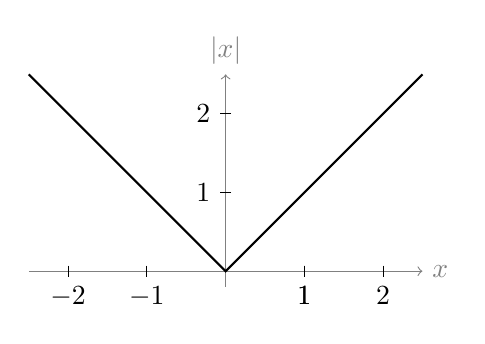
\begin{tikzpicture}[scale=1]
	\draw[->, gray] (-2.5,0) -- (2.5,0) node[right] {$x$};
	\draw[->, gray] (0,-.2) -- (0,2.5) node[above] {$|x|$};
	
	\foreach \x/\xtext in {-2/-2, -1,1, 1/1, 2/2}
	\draw[shift={(\x,0)}] (0pt,2pt) -- (0pt,-2pt) node[below] {{$\xtext$}};
	
	\foreach \y/\ytext in {1/1, 2/2}
	\draw[shift={(0,\y)}] (2pt,0pt) -- (-2pt,0pt) node[left] {{$\ytext$}};
	
	\draw[thick] (-2.5, 2.5)--(0,0)--(2.5, 2.5);
	\end{tikzpicture}
\end{center}
अतः परिभाषा मोटे तौर पर यह कहती है: आप ऐसे निवेश चुनकर जो~$c$ से $\delta$
से अधिक दूर न हों (अर्थात् $|x - c| < \delta$), अपनी ``त्रुटि'' को
$\epsilon$ से कम (अर्थात् $|g(x) - \ell| < \epsilon$) कर सकते हैं।

सीमा की संकल्पना परिभाषित करने के बाद हम उससे अनंतसूक्ष्म राशियों को पूरी तरह
टाल सकते हैं और निर्धारित कर सकते हैं कि $c$ पर $f$ की प्रवणता इससे दी जाती
है:
\[
	{f}'(c) = \lim_{x \rightarrow 0}\left(\frac{f(c +x) - f(c)}{x}\right) \text{ जहाँ सीमा अस्तित्व में है}।
\]
फिर भी यह समझना महत्त्वपूर्ण है कि हमारी परिभाषा को ``जहाँ सीमा अस्तित्व में
है'' वाली सावधानी क्यों चाहिए। एक सरल उदाहरण के लिए $f(x) = |x|$ पर विचार
करें, जिसका आलेख हमने अभी देखा। स्पष्टतः $f'(0)$ अपरिभाषित है: यदि हम $0$ के
``दाईं ओर से'' निकट आएँ, तो प्रवणता सदा $1$ है; यदि ``बाईं ओर से'' निकट आएँ,
तो प्रवणता सदा $-1$ है; अतः सीमा अपरिभाषित है। इसलिए हम जोड़ सकते हैं कि
फलन~$f$,~$x$ पर \emph{अवकलनीय} तभी और केवल तभी है जब ऐसी सीमा अस्तित्व में
हो।

हमने देखा कि \emph{सीमा} की संकल्पना से अवकलन को कैसे संभाला जाए। इसी
संकल्पना से हम \emph{सतत} फलन का विचार परिभाषित कर सकते हैं। (वास्तव में
बोल्ज़ानो 1817 तक यह समझ चुके थे।) सांतत्य का कॉशी--वाइयरश्ट्रास निरूपण इस
प्रकार है। मोटे तौर पर: कोई फलन~$f$ (किसी बिंदु पर) सतत है यदि फलन के निर्गम
में एक निश्चित मात्रा की परिशुद्धता माँगने पर, फलन के निवेश में एक निश्चित
मात्रा की परिशुद्धता पर बल देकर उसकी प्रत्याभूति दी जा सके। अधिक ठीक-ठीक:
$f$, $c$ पर सतत है यदि $x$ के शून्य की ओर बढ़ने पर $f(c + x)$ और स्वयं
$f(c)$ के बीच का अंतर $0$ की ओर बढ़े। दूसरे शब्दों में: $f$, $c$ पर
\emph{सतत} तभी और केवल तभी है जब $f(c) = \lim_{x \rightarrow c} f(x)$।

इससे आगे बढ़ना हमें वास्तविक विश्लेषण में ले जाएगा, जबकि हमारा विषय समुच्चय
सिद्धांत है। अतः अब हमें रुककर शिक्षा कहनी चाहिए। उन्नीसवीं शताब्दी में
गणितज्ञों ने \emph{सीमा} की कठोर रूप से परिभाषित संकल्पना का आह्वान करके
अनंतसूक्ष्म राशियों के बिना काम करना सीखा।

\end{document}
